\documentclass[10pt]{article}
\usepackage{graphicx,amssymb, amstext, amsmath, epstopdf, booktabs, verbatim, gensymb, geometry, appendix, natbib, lmodern, hyperref, inputenc, titlesec}
\geometry{letterpaper}
%\usepackage{garamond}
\usepackage[table]{xcolor}


\setcounter{secnumdepth}{4}
\titleformat{\paragraph}
{\normalfont\normalsize\bfseries}{\theparagraph}{1em}{}
\titlespacing*{\paragraph}
{0pt}{3.25ex plus 1ex minus .2ex}{1.5ex plus .2ex}
\newcommand*\Title{FRIDGES}
\newcommand*\cpiType{Phase 1 Report}
\newcommand*\Date{October 2015}
\newcommand*\Author{Paul McGurk, Alex McBride,  Daniel Rafferty,        Andrew Mortimer, and Scott Henderson} 
\title{FRIDGES}
\author{Paul McGurk, Alex McBride, Daniel Rafferty, Andrew Mortimer, and Scott Henderson}
\date{\today}
%-----------------------------------------------------------

\usepackage{cpistuff/cpi} % This is what makes your document look like a cpi document.


\begin{document}

\begin{titlepage}
\maketitle
\end{titlepage}

\linespread{1.15} %Set standard document linespacing
\renewcommand{\arraystretch}{1.2} %Set table height spacing

\tableofcontents

\newpage
\section{Introduction}

\subsection{About the Project}
The project is to create a product using an Arduino and/or Raspberry Pi that will be a part of the Internet of things. The Internet of things is about taking everyday objects and embedding them with software, electronics and networking capabilities so that they can sense the environment around them and then send and receive data. The idea, after much thought and discussion will be to create a smart fridge. This idea will not only have a physical benefit to its application but also an environmental one, as from the start the design is centred on trying to reduce food waste and energy consumption.

\subsection{Motivation}
According to statistics from \href{http://www.lovefoodhatewaste.com/content/facts-about-food-waste-1}{LoveFoodHateWaste} (a website run by WRAP - Waste and Resources Action Programme) UK households throw away 7 million tonnes of food every year. One of the main reasons for this is not using the food before it goes out of date. The average cost per household of this food wastage is \pounds 470 per year.

\subsubsection{Environmental Impact}

The same website claims that if this food wastage was reduced to 0, it would be equivalent to taking a quarter of the cars in the UK off the road. According to studies from \href{http://www.lovefoodhatewaste.com/content/love-your-fridge-and-waste-less}{WRAP}, by ensuring our fridges are at the right temperature (between 0 and 5 \degree C), as a country there is a potential of \pounds 200 million to be saved. Apprently, 70\% of fridges are kept too warm, meaning food becomes inconsumable much more quickly.

\subsubsection{Our Goal}

By allowing a user to know more easily when foods are soon to be out of date, we hope to reduce food waste and the environmental impact it has.

\newpage
\section{Assessment of Capabilities}

\subsection{Requirements}

The device we end up choosing must be able to support all the hardware and software we want to incorporate into our smart fridge. One of things we want to be able to support is a touchscreen to allow the user to interact with the fridge directly and on top of this a camera to act as a barcode scanner and then display the product on the screen. Another device that we also want to support is a thermometer that will be positioned inside the fridge allowing us to monitor the temperature in the fridge by taking readings. The final thing our device must have is internet capabilities, this is so that we will be able to set up and run our own Web server for the fridge.

\subsection{Arduino}
The Arduino Uno V3 is a small microcontroller board sporting an ATmega328p processor. It is designed for prototyping embedded products and as a result has good support for driving ICs and other low-level peripherals. The 6 PWM outputs allows analogue components to be operated easily, and the lean 16MHz processor is extremely low power meaning it could potentially be powered from a battery.

\begin{figure}[h]
\centering
\caption{Arduino Uno V3}
\label{Arduino Uno V3}
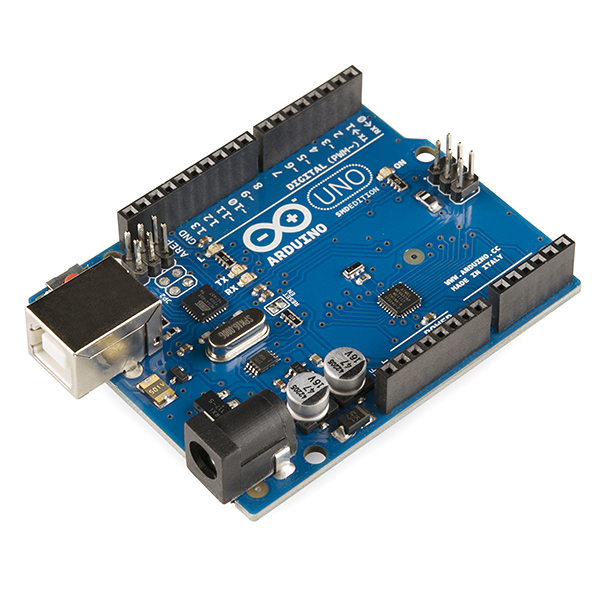
\includegraphics[height=8.5cm]{images/Arduino.jpg}
\end{figure}

\begin{center}
	\rowcolors{1}{white}{gray!15}
	\begin{tabular}{ | c | c | }
		\hline
	 	\multicolumn{2}{|c|}{Arduino Uno V3} \\ \hline
		Microcontroller 	& 16 MHz ATmega328p \\ \hline
		SRAM 			& 2KB \\ \hline
		Flash Memory	& 32KB \\ \hline
		USB 2.0		& None \\ \hline
		HDMI 			& None \\ \hline
		Audio Output	& None \\ \hline
		Digital I/O Pins	& 14 \\ \hline
		Analogue input pins & 6 \\ \hline
	\end{tabular}
\end{center}
\newpage
\subsection{Raspberry Pi}

\begin{figure}[h]
\centering
\caption{Raspberry Pi}
\label{Raspberry Pi}
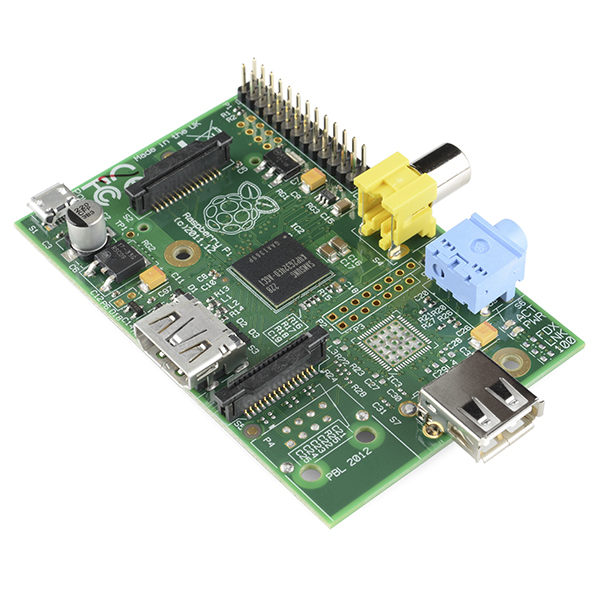
\includegraphics[height=9cm]{images/Raspberry-Pi.jpg}
\end{figure}
The Raspberry Pi is a small form-factor ARM based computer. It is a very popular system that has a healthy development ecosystem. The RPi can run a custom Linux-based operating system, called Raspbian, allowing fairly high level development and integration with lower-level peripherals such as GPIOs. The Raspberry Pi also has official peripherals or "modules" for devices such as a camera or a touchscreen.

There are several models of Raspberry Pi available:

\begin{center}
	\rowcolors{1}{white}{gray!15}
	\begin{tabular}{| c | p{6cm} | p{6cm} |}
		\hline
		  & Raspberry Pi Model A & Raspberry Pi 2 \\ \hline
		CPU & 700 MHz Low Power ARM1176JZ-F Applications Processor & 900MHz quad-core ARM Cortext-A7 \\ \hline
		RAM & 256MB & 1GB \\ \hline
		Ethernet port & None & One \\ \hline
		USB 2.0 & 1 port & 4 ports \\ \hline
		HDMI & Full HDMI port & Full HDMI port \\ \hline
		Audio Output & 3.5mm audio jack & 3.5mm audio jack \\ \hline
		Number of GPIOs & 17 & 40 \\ \hline
	\end{tabular}
\end{center}

\subsection{Choice}
We have chosen to go for the Raspberry Pi 2. The reason we chose a RPi over an Arduino was that we needed the higher performance that the RPi line offers in order to serve our Web pages and do the barcode scanning in software. Furthermore we wanted internet connectivity and we felt this would be easier to achieve in the Linux based Pi. The reason we chose to use the model 2 instead of the model A was the better connectivity for peripherals in terms of USB ports and available GPIOs, with the higher performance an added bonus.

\newpage
\section{Hardware Design}
\subsection{Main Parts}
\subsubsection{RGB LED}

An RGB LED (Red Green Blue Light Emitting Diode) is a small light which has three different diodes within it, capable of emitting three types of light. Each pin controls a different colour, with the longest pin being the PLUS. Using PWM (Pulse Width Modulation), we can dim and lighten the different colours to give a range of colours. The operating temperature of the LED covers the expected temperature in the fridge.

This is being used within the project as a visual display of the temperature in the fridge, with blue representing when the reading is near the ideal temperature, and red when it is too warm.

\begin{figure}[h]
\centering
\caption{RGB LED}
\label{RGB LED}
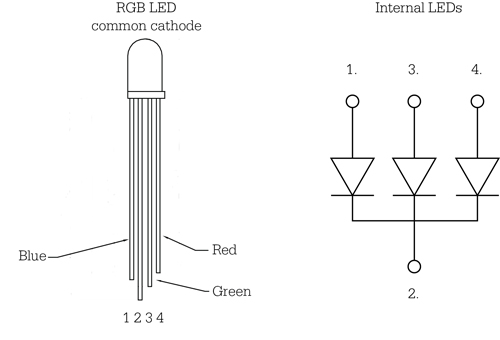
\includegraphics[height=5cm]{images/rgb_led_diagram.jpg}
\end{figure}

\begin{center}
	\rowcolors{1}{white}{gray!15}
	\begin{tabular}{|*{6}{c|}}
		\hline
		\textbf{Colour} & Wave Length & Forward Voltage & Forward Current & Luminosity & Operating Temperature \\ \hline
		Red & 623nm & 2.0V & 20ma & 2800mcd & -25 \textasciitilde \ 85\degree C \\ \hline
		Green & 517.5nm & 3.2V & 20ma & 6500mcd & -25 \textasciitilde \ 85\degree C \\ \hline
		Blue & 466nm & 3.2V & 20ma & 1200mcd & -25 \textasciitilde \ 85\degree C \\ \hline
	\end{tabular}
\end{center}

\subsubsection{Resistor}

A resistor is a device which reduces the flow of current within a circuit. This can be used for many applications such as protecting elements from high current.

This is being used within the project to protect the RGB LED, as a pull-up for the hall effect sensor, and within the temperature part of the circuit to work out the resistance of the thermistor (see below).

\begin{figure}[h]
\centering
\caption{Resistor}
\label{Resistor}
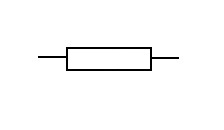
\includegraphics[height=2cm]{images/resistor_diagram.jpg}
\end{figure}

\begin{center}
	\rowcolors{1}{white}{gray!15}
	\begin{tabular}{|c|c|}
		\hline
		Value & Quantity \\ \hline
		10k\ohm & 1 \\ \hline
		1k\ohm & 2 \\ \hline
		470\ohm & 3 \\ \hline
	\end{tabular}
\end{center}

\subsubsection{Thermistor}

A thermistor is a resistor which is sensitive to temperature. The resistance of the thermistor is used to work out the temperature of it's surroundings via the Steinhart-Hart equation.

This is being used within the project to work out the temperature within the fridge, allowing us to monitor it in real-time.

\begin{figure}[h]
\centering
\caption{Thermistor}
\label{Thermistor}
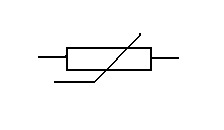
\includegraphics[height=2.5cm]{images/thermistor_diagram.jpg}
\end{figure}

\begin{center}
	\rowcolors{1}{white}{gray!15}
	\begin{tabular}{|c|c|}
		\hline
		Value & Quantity \\ \hline
		1k\ohm \ (at 25\degree C) & 1 \\ \hline
	\end{tabular}
\end{center}

\subsubsection{Capacitor}

A capacitor is a device which stores electrical energy temporarily.

This is used within the project to work out the temperature of the fridge, which is done by measuring how long it takes to drain the capacitor, with the resistance of the thermistor being dependent on the temperature.

\begin{figure}[h]
\centering
\caption{Capacitor}
\label{Capacitor}
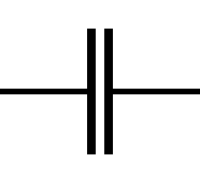
\includegraphics[height=2.5cm]{images/capacitor_diagram.jpg}
\end{figure}

\begin{center}
	\rowcolors{1}{white}{gray!15}
	\begin{tabular}{|c|c|}
		\hline
		Value & Quantity \\ \hline
		330nF & 1 \\ \hline
	\end{tabular}
\end{center}

\subsubsection{Hall Effect Sensor and Magnet}

A Hall Effect sensor detects magnetic fields. It is often used as a non-contact switch for applications such as doors. We intend to mount the sensor on the chassis of the fridge next to the door, and mount a magnet on the door itself, aligned with the sensor. When the door is closed the sensor will detect the magnetic field from the magnetic and the output signal will go low. When the door is opened, the magnetic field will not be detected by the sensor and the signal will go high.

\begin{figure}[h]
\centering
\caption{Hall Effect Sensor}
\label{Hall Effect Sensor}

\includegraphics[width=8cm]{images/hall-effect-sensor.jpg}
\end{figure}

\subsubsection{Raspberry Pi Camera}

The Raspberry Pi Camera Board connects to any Raspberry Pi and allows for high definition photography. It has several useful features, including: high data capability, 5 mega-pixel fixed focus, support for 1080p, 720p60 and VGA90. It also has automatic control functions including white balance, exposure control, and luminance detection.
The Pi Camera Board has a 15cm ribbon cable which slots into the Pi Camera Serial Interface Port. Via Raspbian, there are several applications that can be used to take photos, including Raspistill.

\begin{figure}[h]
\centering
\caption{Raspberry Pi Camera}
\label{Raspberry Pi Camera}
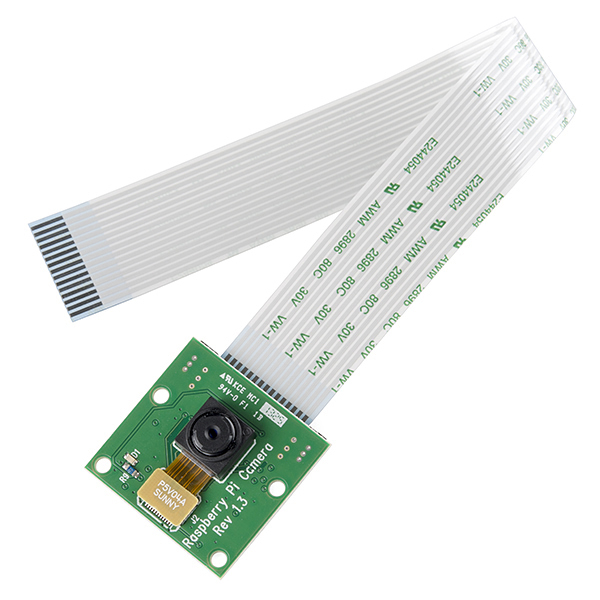
\includegraphics[height=4cm]{images/pi-camera.jpg}
\end{figure}

\begin{center}
	\rowcolors{1}{white}{gray!15}
	\begin{tabular}{ | c | c | }
		\hline
	 	\multicolumn{2}{|c|}{Technical Specifications} \\ \hline
		Dimensions 		& 8.5 x 8.5 x 5mm \\ \hline
		Maximum frame rate capture 	& 30fps @ 1080p, 60fps @ 720p \\ \hline
		Maximum supported resolution	& 2592 x 1944 \\ \hline
		Supported Bus Interfaces		& I2C \\ \hline
		Supported Video Ports		& Raspberry Pi \\ \hline
		Minimum Operating Temperature	& -30\degree C \\ \hline
	\end{tabular}
\end{center}

The minimum operating temperature of -30\degree C means we could mount the camera inside the fridge if we so desire.

This will be used within the project to scan the barcode of the products being entered into the fridge. It could possibly automatically detect the use-by date as well.

\newpage
\subsubsection{Raspberry Pi Touch Screen Display}

The Raspberry Pi 7" Touchscreen Display connects to a Raspberry Pi, and allows it to display graphics in a self-contained package. It also allows the user to interact with the GUI through touch, omitting the need for additional peripherals such as mouse and keyboard.

We chose this screen because other options were too small to be able to display a useful amount of information and still be able to type on.

\begin{figure}[h]
\centering
\caption{Raspberry Pi Touchscreen}
\label{Raspberry Pi Touchscreen}
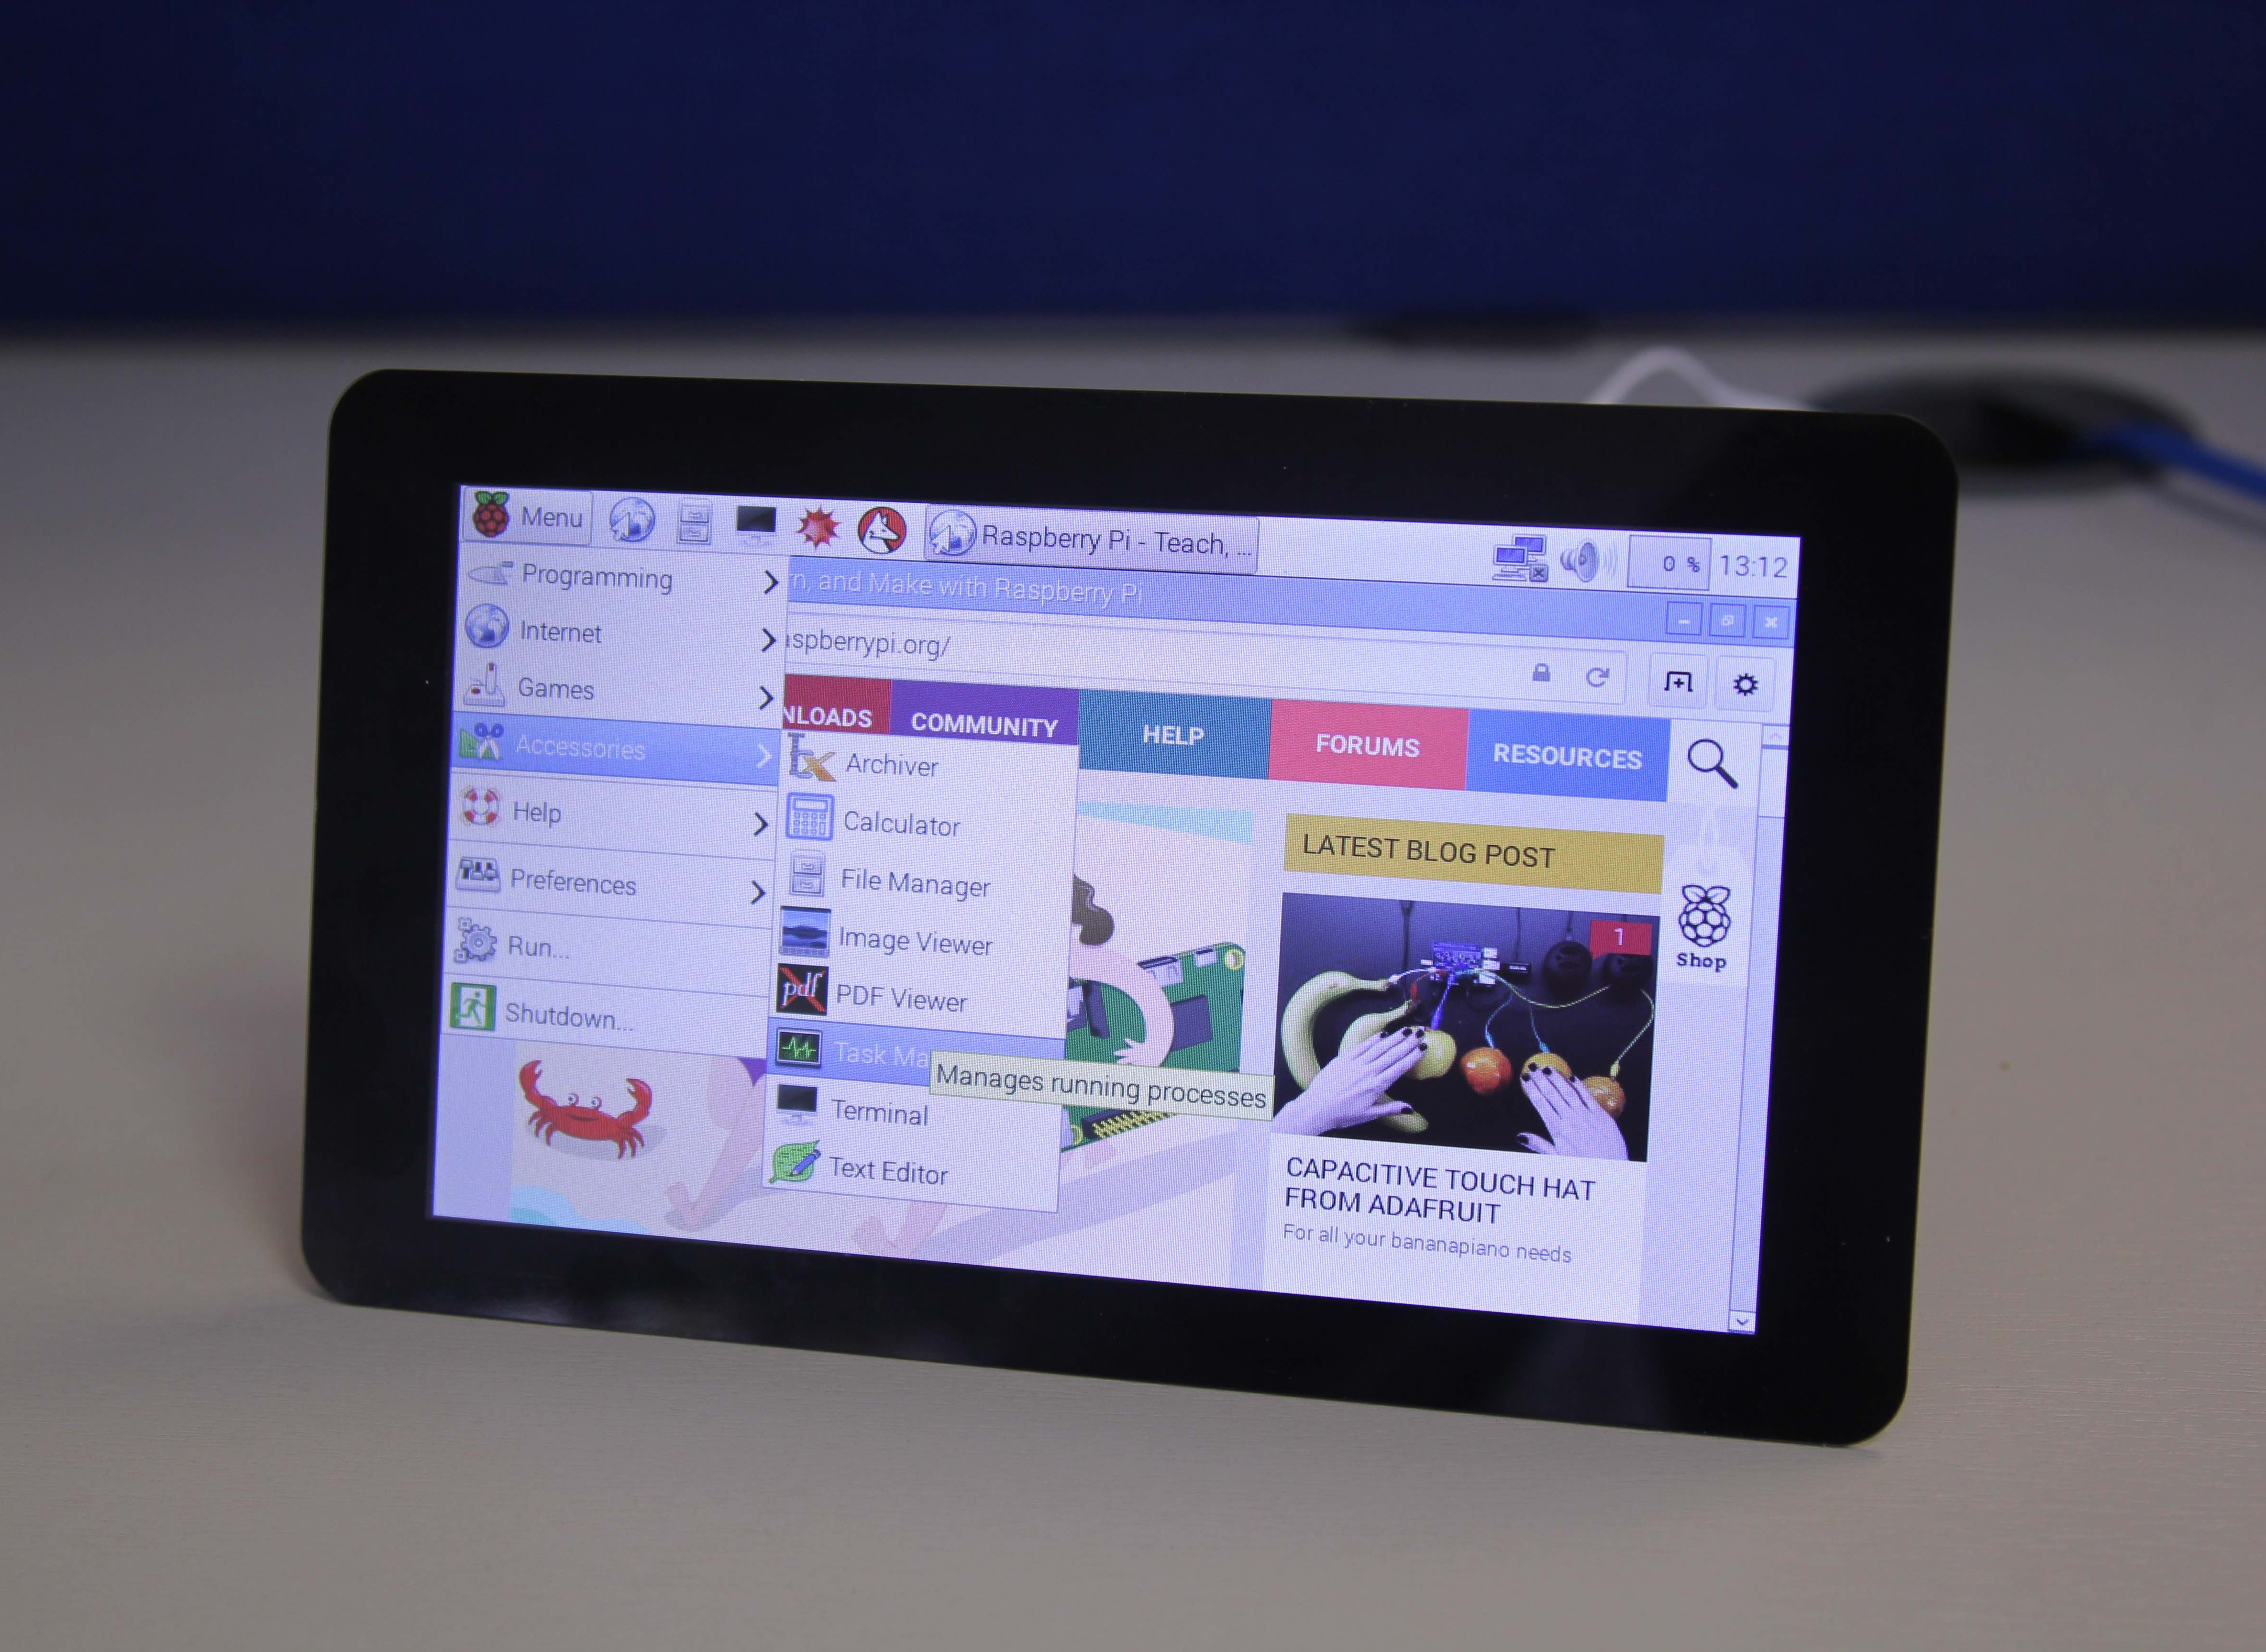
\includegraphics[height=7cm]{images/pi-touchscreen.jpg}
\end{figure}

\begin{center}
	\rowcolors{1}{white}{gray!15}
	\begin{tabular}{ | c | c | }
		\hline
	 	\multicolumn{2}{|c|}{Technical Specifications} \\ \hline
		Dimensions 		& 194mm x 110mm x 20mm \\ \hline
		Viewable screen size 	& 155m x 86mm \\ \hline
		Screen resolution	& 800 x 480 \\ \hline
	\end{tabular}
\end{center}

This will be used within the project to display a custom GUI which will have a number of uses, such as; display all products which are near their use-by date, adding custom products (homemade food, products which do not scan properly, etc). From this screen, the user will also be able to see the temperature of the fridge, and possibly configure the Web server.

\subsection{Component List}
\begin{center}
	\rowcolors{1}{white}{gray!15}
	\begin{tabular}{ | c | c | c | c |}
		\hline
	 	Quantity & Component Name & PriceUnit & Total Price \\ \hline
		1	& Raspberry Pi Touch Screen 	& \pounds 42.99	& \pounds 42.99 \\ \hline
		1 	& Raspberry Pi Camera 	& \pounds 16.20	& \pounds 16.20 \\ \hline
		1	& 330nF Capacitor	& \pounds 0.09	& \pounds 0.09 \\ \hline
		1	& RGB LED   & \pounds 2.76	& \pounds 2.76 \\ \hline
		1	& Thermistor	& \pounds 0.60	& \pounds 0.60 \\ \hline
		1	& 10k\ohm & \pounds 0.053 	& \pounds 0.053 \\ \hline
		2	& 1k\ohm & \pounds 0.027	& \pounds 0.054 \\ \hline
		3	& 470\ohm & \pounds 0.005	& \pounds 0.02 \\ \hline
		1	& Digital Hall Effect Sensor & \pounds 1.53	& \pounds 1.53 \\ \hline
		1	& Magnet & \pounds 1.055	& \pounds 1.055 \\ \hline
			& 	& Total 	& \pounds 65.37 \\ \hline
	\end{tabular}
\end{center}

\newpage
\subsection{Prototype Temperature Circuit}
To accurately assess the feasibility of certain parts of this project, we created a prototype circuit of the temperature sensitive LED component. This was completed with a breadboard connecting the GPIO pins to a range of devices, most notable of which being a thermistor, and a RGB LED.

\subsubsection{Circuit Diagram}
\begin{figure}[h]
\centering
\caption{Prototype Circuit}
\label{Prototype Circuit}
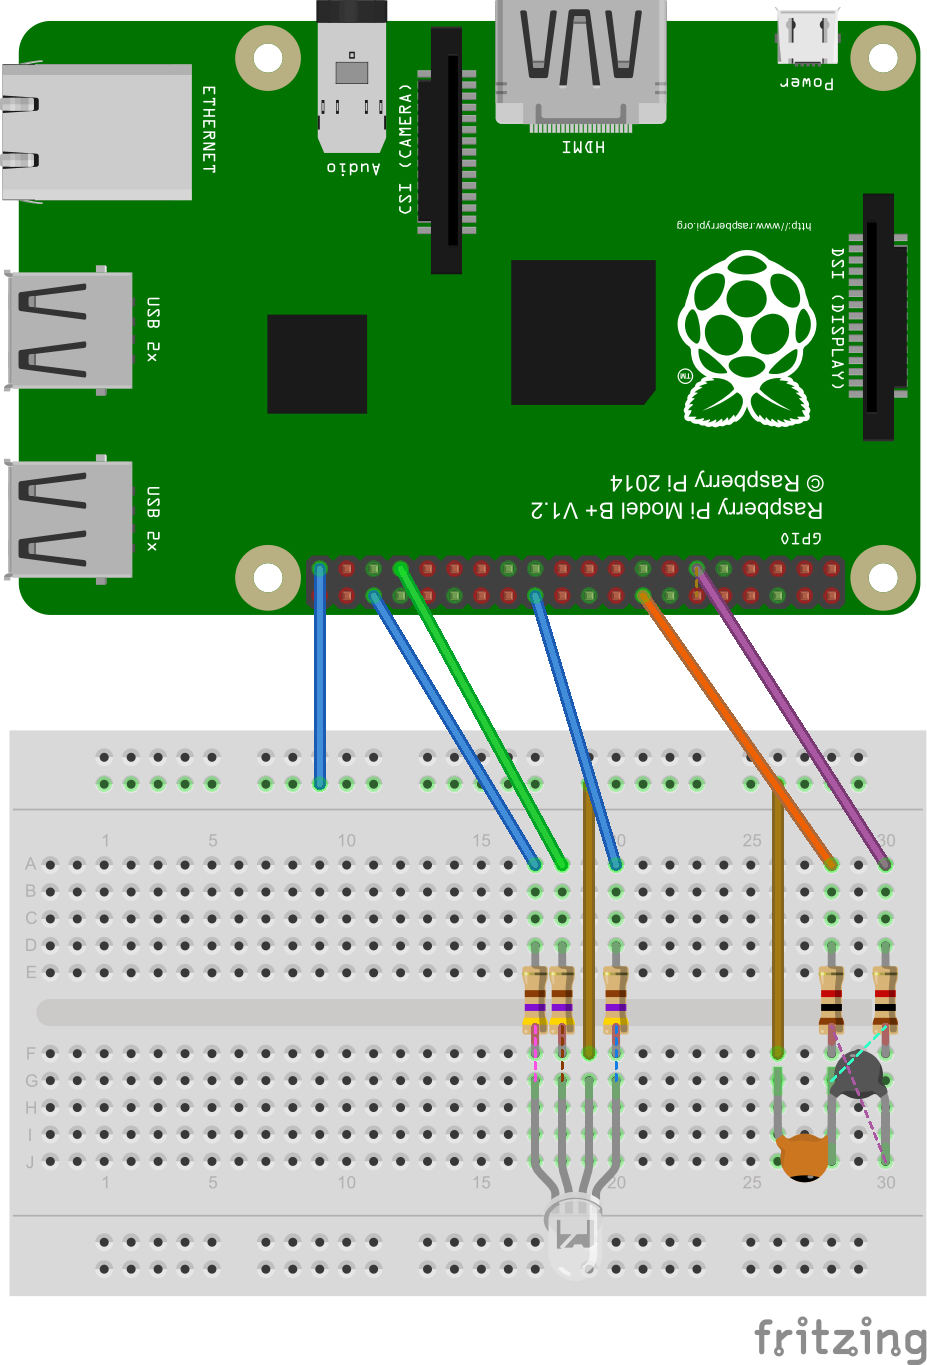
\includegraphics[height=8cm]{images/prototypeDiagram.png}
\end{figure}

\subsubsection{Result}
\begin{figure}[h]
\centering
\caption{Prototype working}
\label{Prototype working}
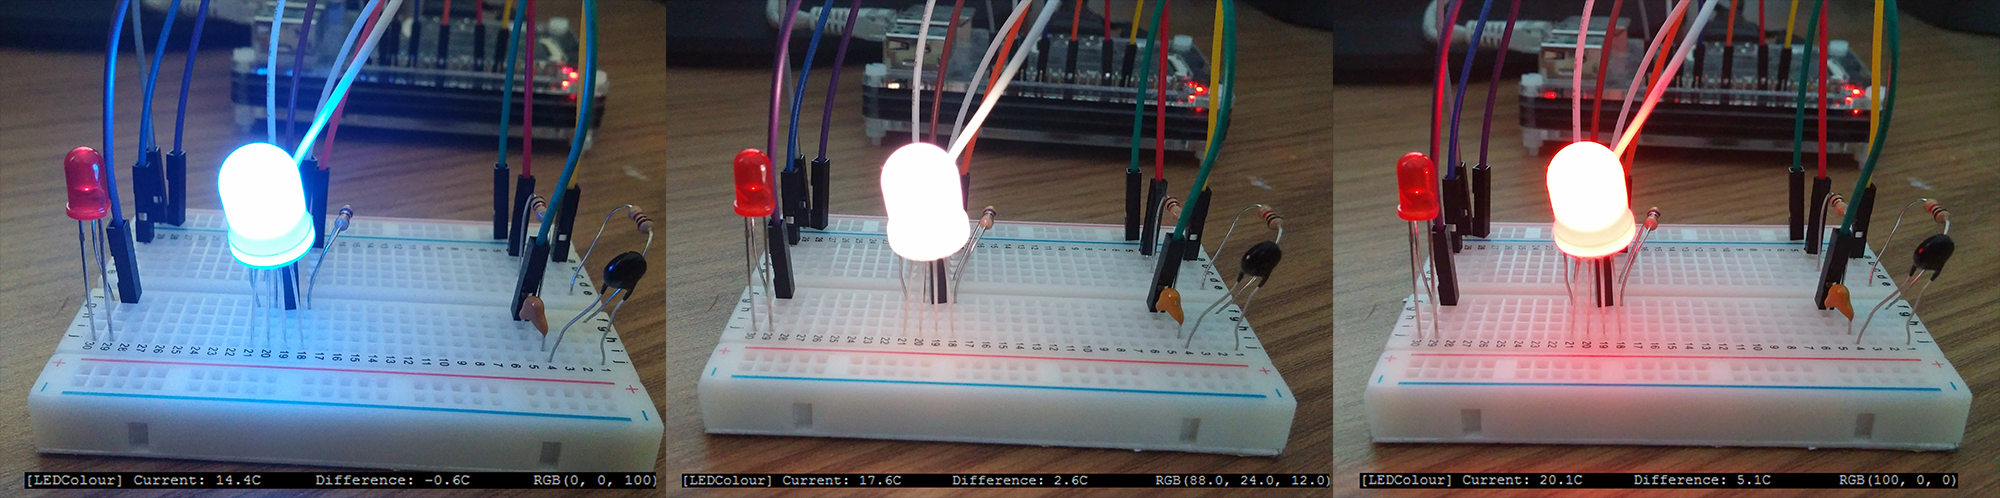
\includegraphics[height=4cm]{images/tempsenproto.png}
\end{figure}
\pagebreak
\subsection{Prototype Door State Circuit}

The prototype for detecting the state of the door consists of a breadboard, the hall effect sensor and magnet, and a resistor. We could do away from the breadboard since it is attached almost directly to the Pi.

\subsubsection{Circuit Diagram}
\begin{figure}[h]
\centering
\caption{Prototype Circuit}
\label{Prototype Circuit}
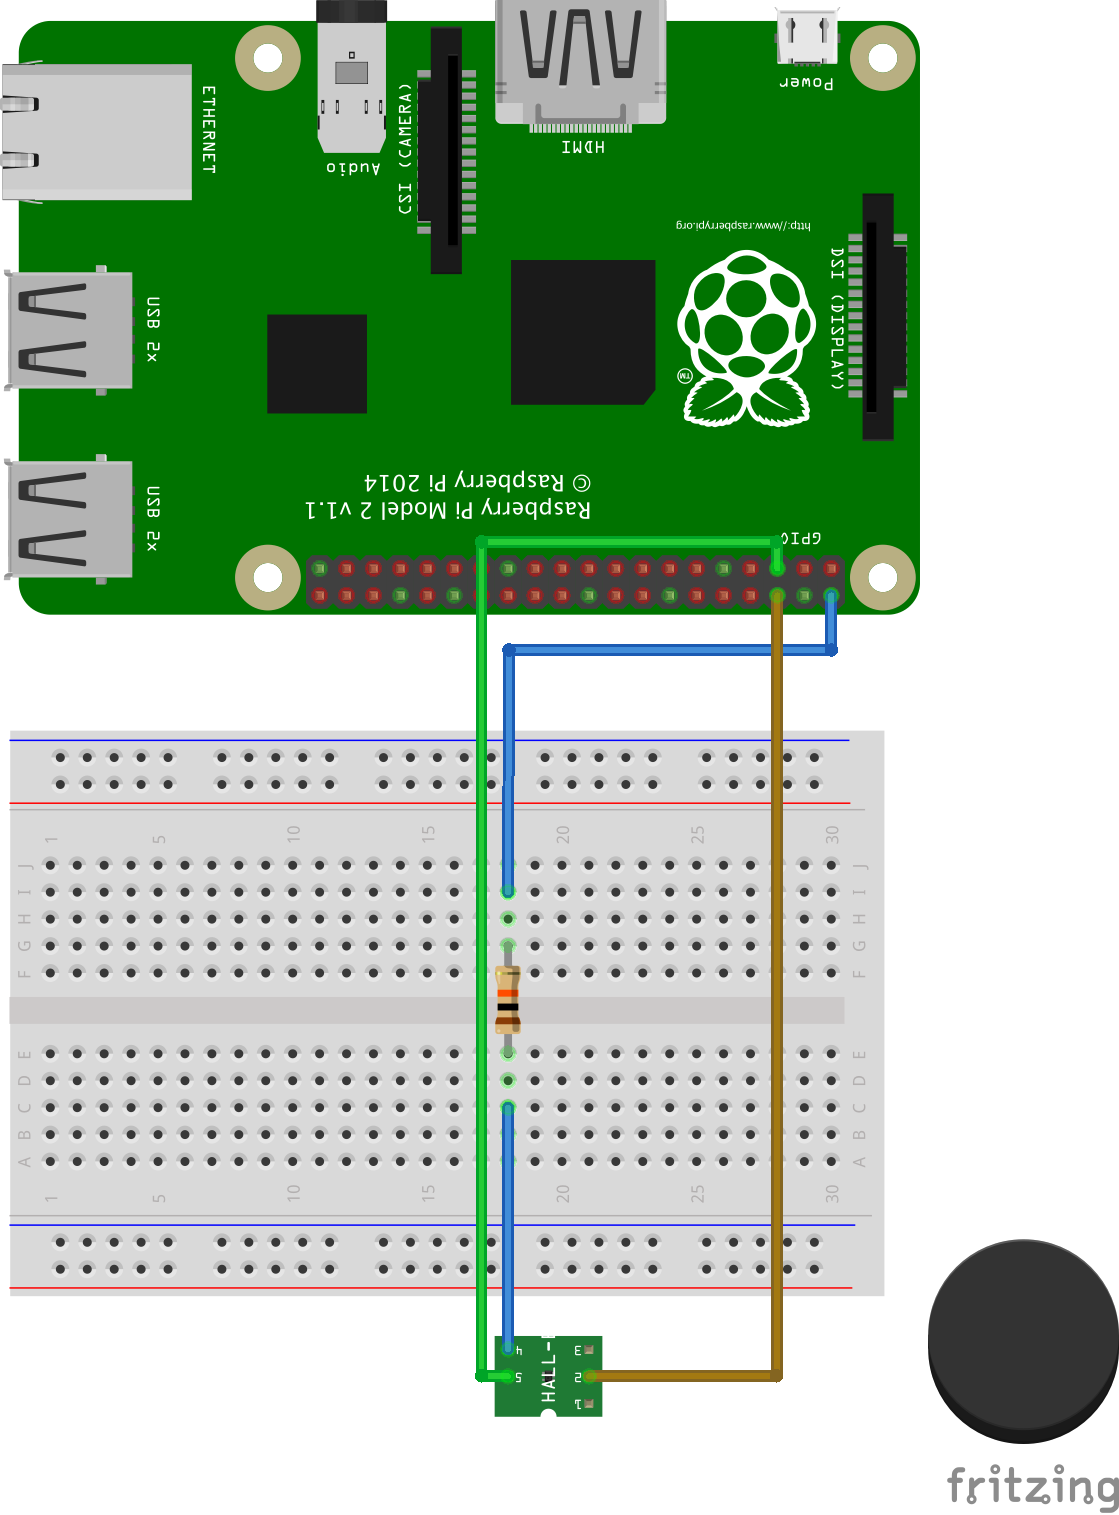
\includegraphics[height=8cm]{images/hall_effect_diagram.png}
\end{figure}

\subsubsection{Circuit Schematic}
\begin{figure}[h]
\centering
\caption{Prototype Circuit Schematic}
\label{Prototype Circuit Schematic}
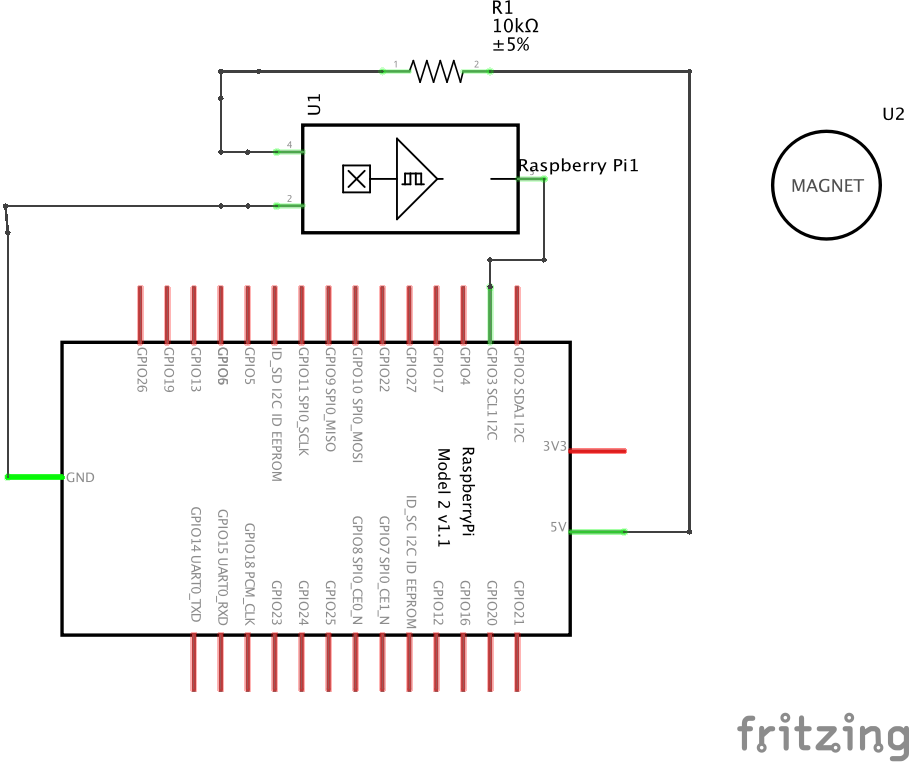
\includegraphics[height=6cm]{images/hall_effect_schem.png}
\end{figure}

\newpage
\section{Software Design}
\subsection{Operating System}
\href{https://www.raspbian.org/}{Raspbian} is a Linux Debian-based operating system which is designed to run on a Raspberry Pi. It optimizes the full power of the Linux desktop environment for the Raspberry Pi's hardware. It allows us to focus on writing the functionality of the software that is unique to our smart fridge, leveraging the rich software ecosystem of 35000 packages that are offered by Raspbian to implement some of the more "standard" technologies such as the Web server.

\subsection{Accessing the hardware}
\href{https://pypi.python.org/pypi/RPi.GPIO}{RPi.GPIO} is a library that allows high level access to the GPIOs on the board through python bindings. Since we currently do not have plans to utilize the hardware PWM, SPI, or I2C functionalities we are not limited by the fact that RPi.GPIO does not support these. If we choose to use any of these functionalities then we can implement them in C and call down from Python fairly easily.

\subsection{Web server}
\subsubsection{Why use a Web Server?}

Most of the functionality of our project requires us to have an interface to the fridge to administrate and view information. We have chosen to go with a Web-based approach, with the RPi itself hosting the Web server. Going with this approach allows us to write the client application once and access it from a phone or a desktop without having to write client applications directly for each.

\subsubsection{Technology Stack}

Since the RPi.GPIO library provides access to the GPIOs via Python, we thought it prudent to serve the dynamic content of our application from Python also. However, we had originally implemented the server using Apache and PHP5, so we had to change this to a Python-based approach. We achieved this using the \href{http://flask.pocoo.org/}{Flask} framework. Flask features a Web server and a templating engine to allow us to write static HTML with wildcards that allow us to dynamically insert relevant data. This also allows us to access the sensors on the Pi to provide the user with up-to-date data straight from the fridge. Although none of us had any experience with this technology before, we thought it was a natural fit and did not have too much trouble implementing it.

\subsection{Temperature Measurement}

The temperature measurement element of this project is currently written in Python. This program was modified from a script written by Simon Monk for his ``Raspberry Pi Starter Pack''. The program works by measuring the time it takes to empty a 330nF capacitor, using the variable resistance from the thermistor, which depends on the temperature. 

\newpage
\subsection{Barcode Scanning}
\subsubsection{Barcode Scanning Library}

\href{http://zbar.sourceforge.net/}{Zbar} is an open source barcode reading library that supports a wide range of barcode formats. It has Python bindings allowing us to read the barcodes in Python.

\subsubsection{Identifying Products using the Barcode}


\href{https://www.outpan.com/}{Outpan} is a web service that provides an API for identifying products from their GTIN. It is free to use and has a database of millions of products. We can make simple HTTP requests with the barcode we just scanned and get information such as the name of the product back.

\subsection{Door State Detection}

Using the hall effect sensor attached to a GPIO, we will be able to use the RPi.GPIO library to detect whether the door is open or closed. This information might be tied in with the temperature measurement in order to indicate to a user when they are leaving the fridge door open for too long.

\newpage
\subsection{Interface}
\subsubsection{Local}
The touchscreen interface will be written in HTML5, JavaScript and CSS3, using the Materialize CSS for the visuals. As for the keyboard for entering data, we will use \href{https://github.com/xlab/matchbox-keyboard}{Matchbox keyboard.}

\begin{figure}[h]
\centering
\caption{Touchscreen GUI flow}
\label{Touchscreen GUI flow}
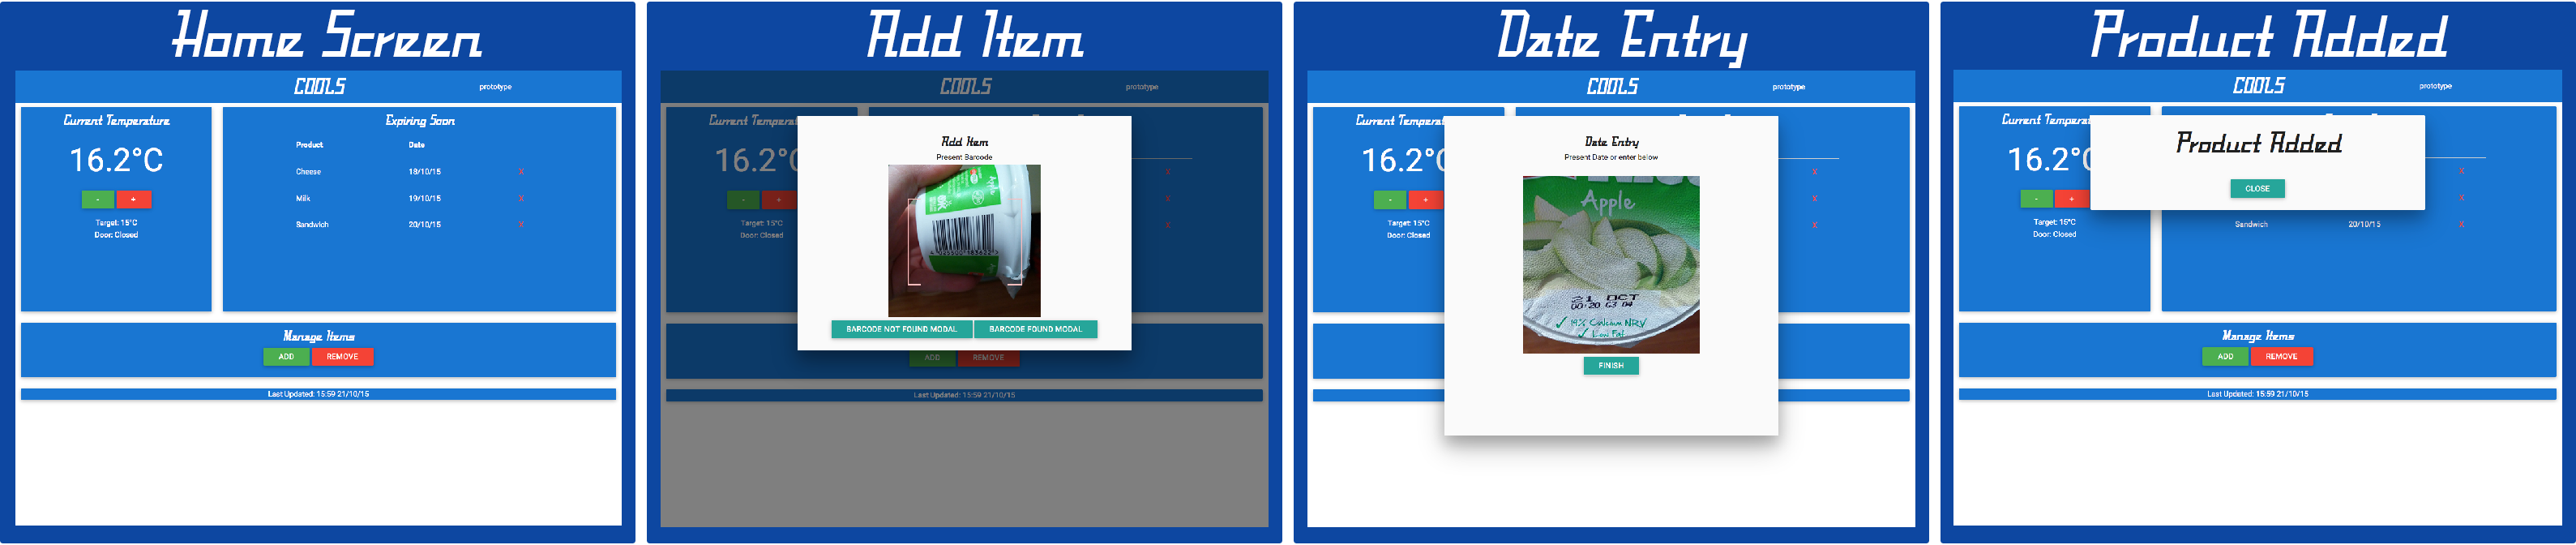
\includegraphics[width=18cm]{images/GUI-flow.png}
\end{figure}


\subsubsection{Remote}

The mobile interface will also be written in HTML5, JavaScript and CSS3, again, using the Materialize CSS library. This interface will be similar to the touchscreen interface, visually, but will not be able to add products, at least to begin with.

\begin{figure}[h]
\centering
\caption{Remote GUI accessed on a Mobile}
\label{Remote GUI accessed on a Mobile}
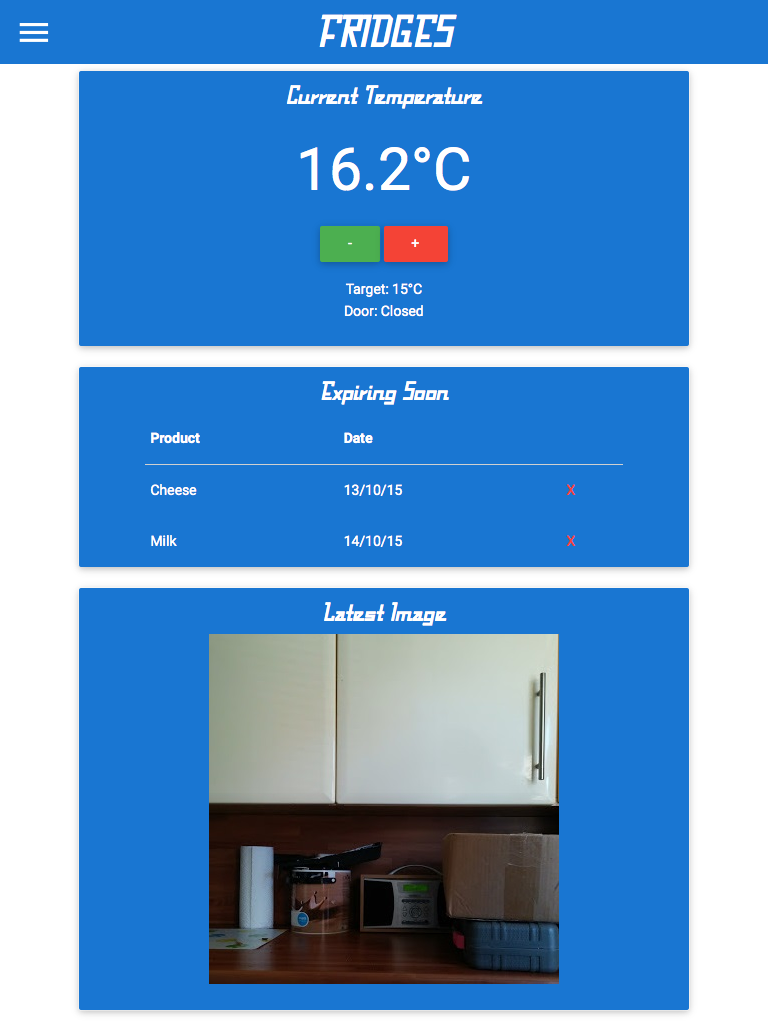
\includegraphics[height=10cm]{images/Mobile-Screenshot.png}
\end{figure}

\section{GANTT Chart}
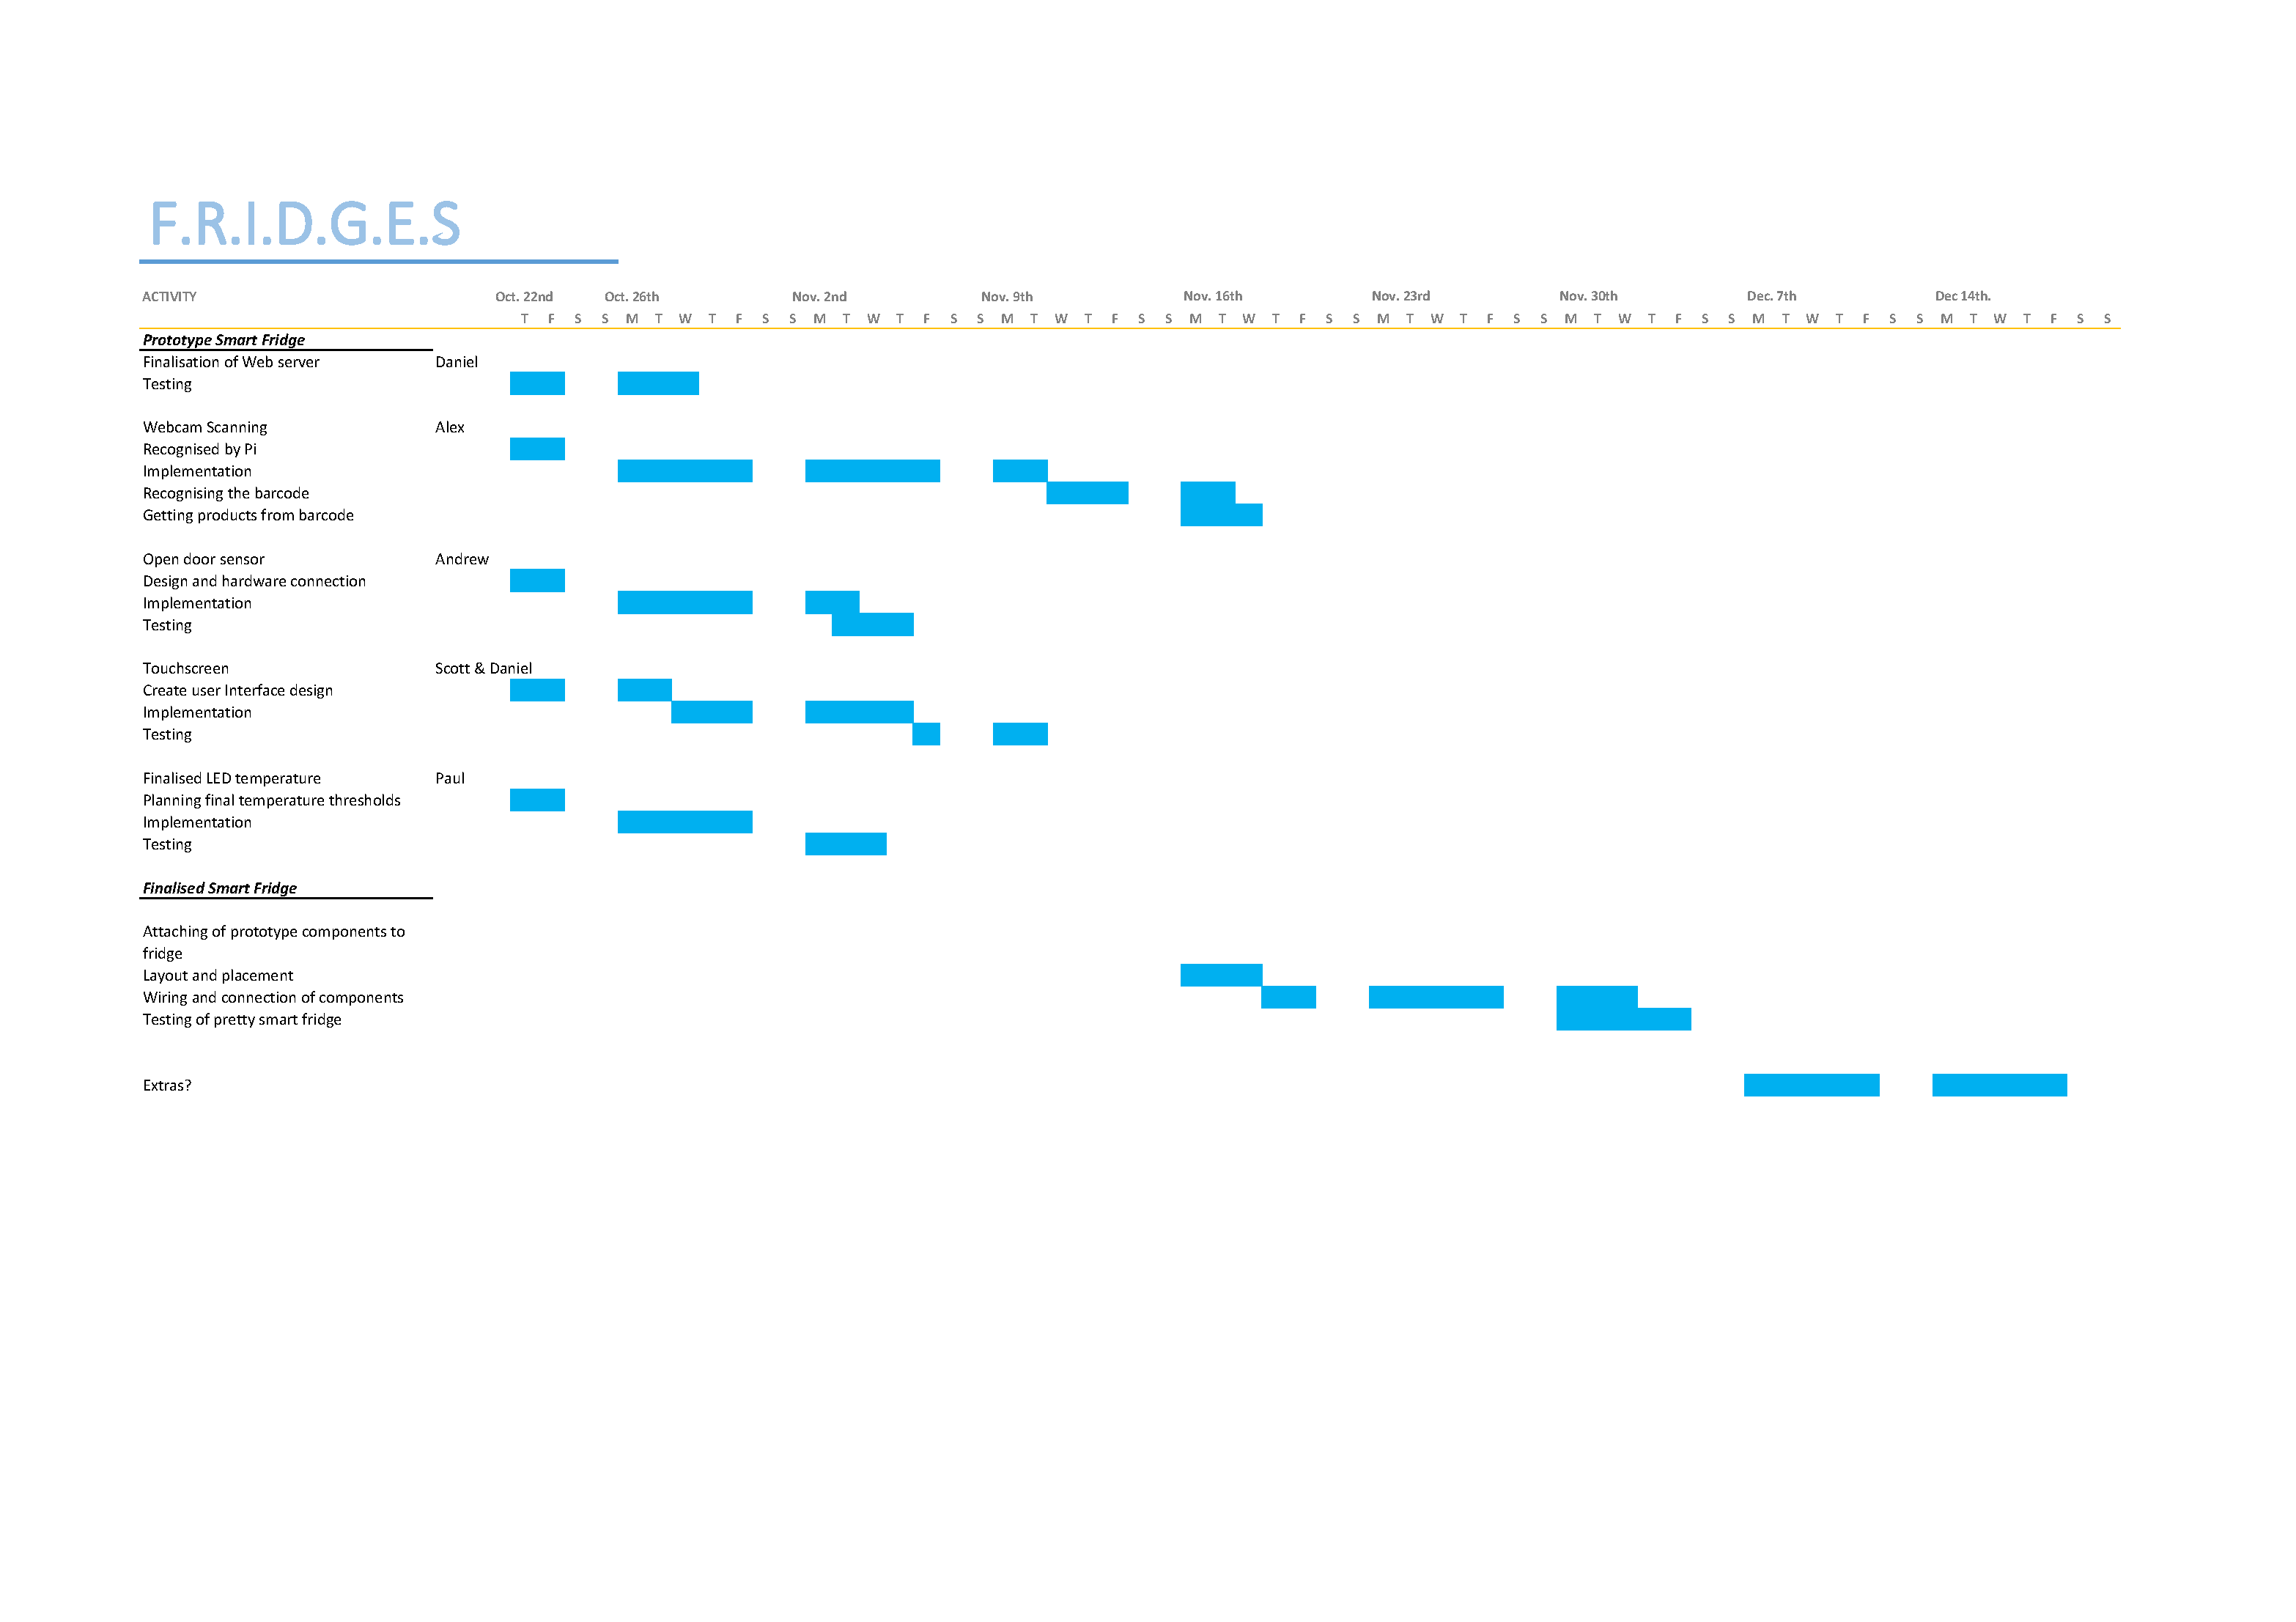
\includegraphics[height=24cm, width=24cm,angle=90]{GANTT.pdf}

\newpage

\section{Organisation}
To organise our group we used a few online tools. We are using a \href{https://github.com/pmcgurk/CS413}{GitHub} repository to keep track of changes in our code and to allow multiple people to work on the same file. With Git, we can see who is working on each part of the project, preventing people from doing the same part accidentally or doing nothing at all. This will also give us version control in case we have to roll back to a previous part of the project.

We are also using the project management application Trello. This enables us to assign members of the group to different "tasks" and keep track of what we have already done. This also allows us to keep track of due dates so our work will always be on time. Trello's commenting system means we can communicate easily as a group, without having to email everyone separately. This is useful as communication is one of the most important aspects of group organisation.

\section{Current Progress}

Our excellent group organisation has allowed us to have already made good progress on Phase 1 of our project. To begin with, we have researched all of the necessary components to complete our project, including deciding on a Raspberry Pi 2 as the basis for our embedded system. We have also created a demo to sense temperature and change the colour of an LED using this Pi, as this is one of the main features of our project. Another feature that we have already implemented is a Flask Web server running on the Pi. Flask will give us an easy way to store data and check the values of the sensors remotely via a Web interface. We have also planned a prototype that will allows us to identify the major challenges in our design/software before moving onto the final build of our project. The basis of a Web interface has been created to allow a user to view temperature, display current contents of the fridge (including expiration dates), and also to show the latest image from the Pi camera.

\section{Stretch Features}
If we meet all of our deadlines, there are some extra features we would like to implement. One of these features would be for the user to be able to change the temperature of the fridge from both the touch interface and remotely. This would be useful as it would give the user greater control over the fridge and enhance the energy saving aspects of the fridge.

One other feature would be to recommend meals based on what is currently in your fridge. These meals could be taken from an open-source recipe database, like \href{http://api.bigoven.com}{Big Oven}, and can be filtered based on what may be going out of date in your fridge. This further reduces food wastage.

Ordering more food would also be a great feature to aid in food reduction. The fridge could recognise when you are low on a specific product, and order more for you from your preferred supplier (Asda/Tesco/Amazon). This would result in less over-buying, as more food would only be ordered when the current stock is low.

User profiles are another optional feature we would like to add. This would allow a group of users (families, housemates) to mark which food is theirs, and receive personalised information. This would also allow user customisation, like changing the interface colours/backgrounds. This would also allow us to have the fridge only open for recognised users, either by login or NFC chip.

Our final extra feature would be to allow users to add widgets to the interface of their fridge. These could include Reminders, Weather forecasts, Daily News and even information from Twitter/Facebook feeds. 

\section{Conclusion}

We have outlined a solid plan to go forward and start developing our smart fridge. By staying as organised as we have been so far, we should meet all the deadlines (submission ones as well as ones we have set ourselves) with no trouble. Building a smart fridge will be very interesting, not only because we will have a useful product by the end of the project, but also because of the environmental implications. By being able to monitor the temperature of the fridge, as well as alerting a user if the door has been left open, we will ensure the fridge will use the least amount of power possible. Secondly, by giving the user an obvious visual representation of which foods are going out of date soon, there is the hope that this will reduce food wastage. Furthermore, it is generally a useful system which will be applicable to the real world. We look forward to making good progress, and our strong group dynamic will allow us to overcome any obstacles with minimal stress.
\end{document}